\Chapter{Kamerapozíció becslése a virtuális térben}

\Section{Markerek}

\SubSection{Klasszikus markeres megoldások}\\
A kiterjeszetett valóság fontos eszköze a marker, ami a model/modellek térben való elhelyezésében segít. Számos nyílt forráskodú könytár rendelkezésre áll a klasszikus értelemben vett markerekből.\\

{\bf Vonalkód, QR-kód:}\\
„A  QR  kód vagyis Quick  Response  (gyors  válasz) egy  mátrix  vonalkód,  vagy  más  néven kétdimenziós kód, mely intelligensebb, több információt hordoz magában a vonalkódoknál: míg egy vonalkód mintegy 13 számjegyet tárol, addig a QR kód 7000 számot és 4300 alfanumerikus karaktert illetve weboldalak címeit (URL),nagy terjedelmű szöveget és telefonszámokat is képes tárolni, bármilyen nyelven.”\\

\begin{figure}[htp]
    \centering
   	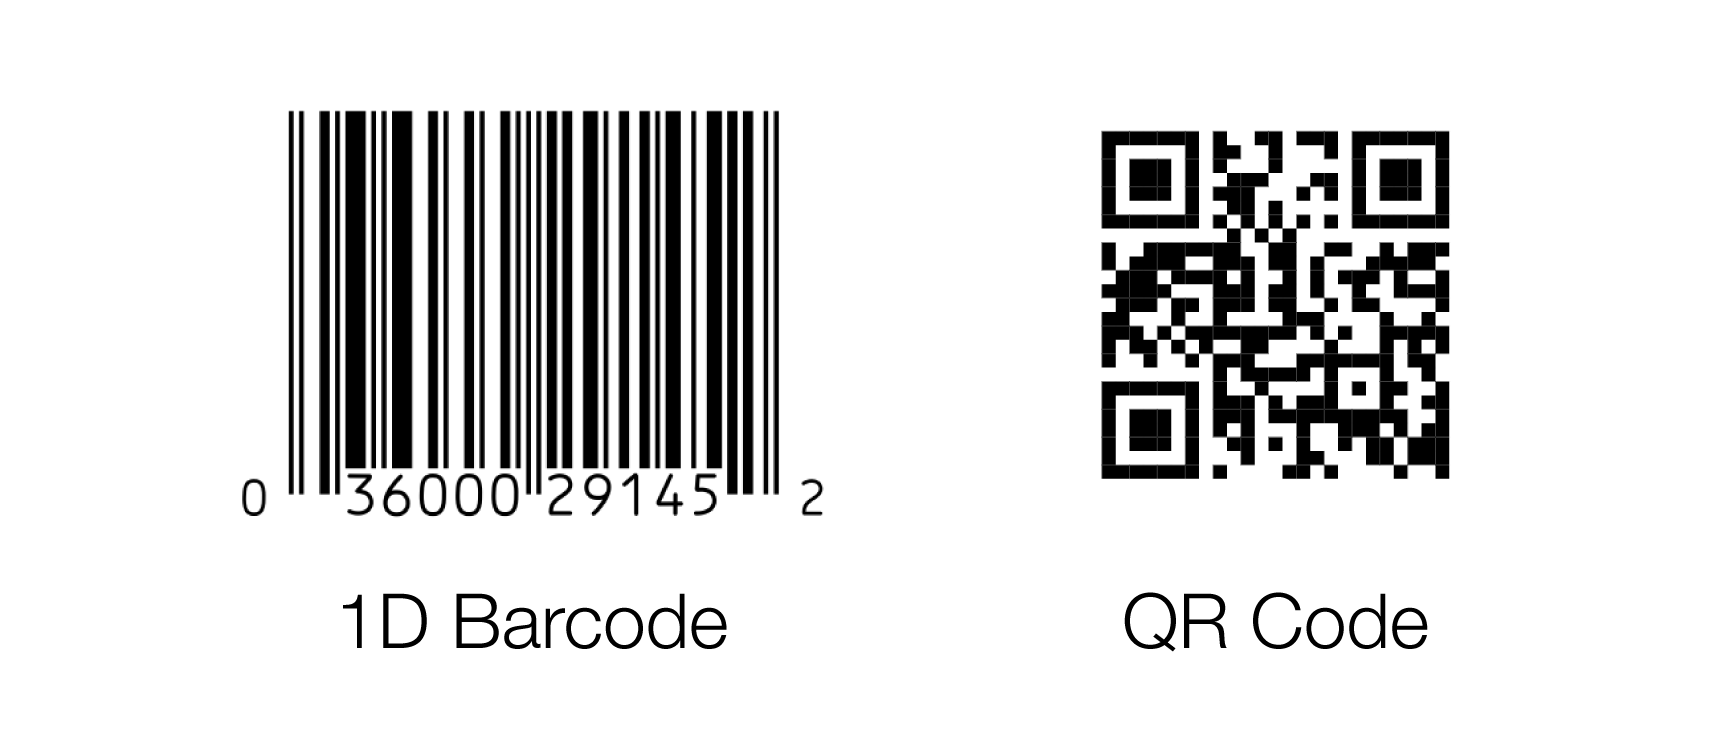
\includegraphics[width=4.8truecm, height=2truecm]{images/qr_bar.png}
	\caption{Vonalkód, QR-kód}
\end{figure}

{\bf „Keretes” markerek:}

Az ilyen típusú markerek két részből állnak; egy fekete keretből, ami a felismerést segití és egy belső mintából. A belső minta lehet kép, egyedi bináris minta.

A keret fontos szerepet tölt be, hisz egy fekete téglalapot/négyzetet viszonylag egyszerűen és gyorsan fel lehet ismerni egy képen, meghatározni annak pozícióját a kamerához képest, sarok pontjait, a középpontját.

Ilyen típusú marker az ARToolKit marker (középen egy kép van, ami bináris képként lesz kezelve), ARTag, AprilTag, ArUco. (mindháromnál egy bináris minta van középen)

Kombinálni is szokták az egyszerűbb markereket: a QR-kódot és a kerettel rendelkező markereket, vagy a QR kód van a keret belsejében vagy pedig a QR kód közepén szerepel például egy ArUco marker vagy egy kép (pl.VuMark).

\begin{figure}[htp]
    \centering
   	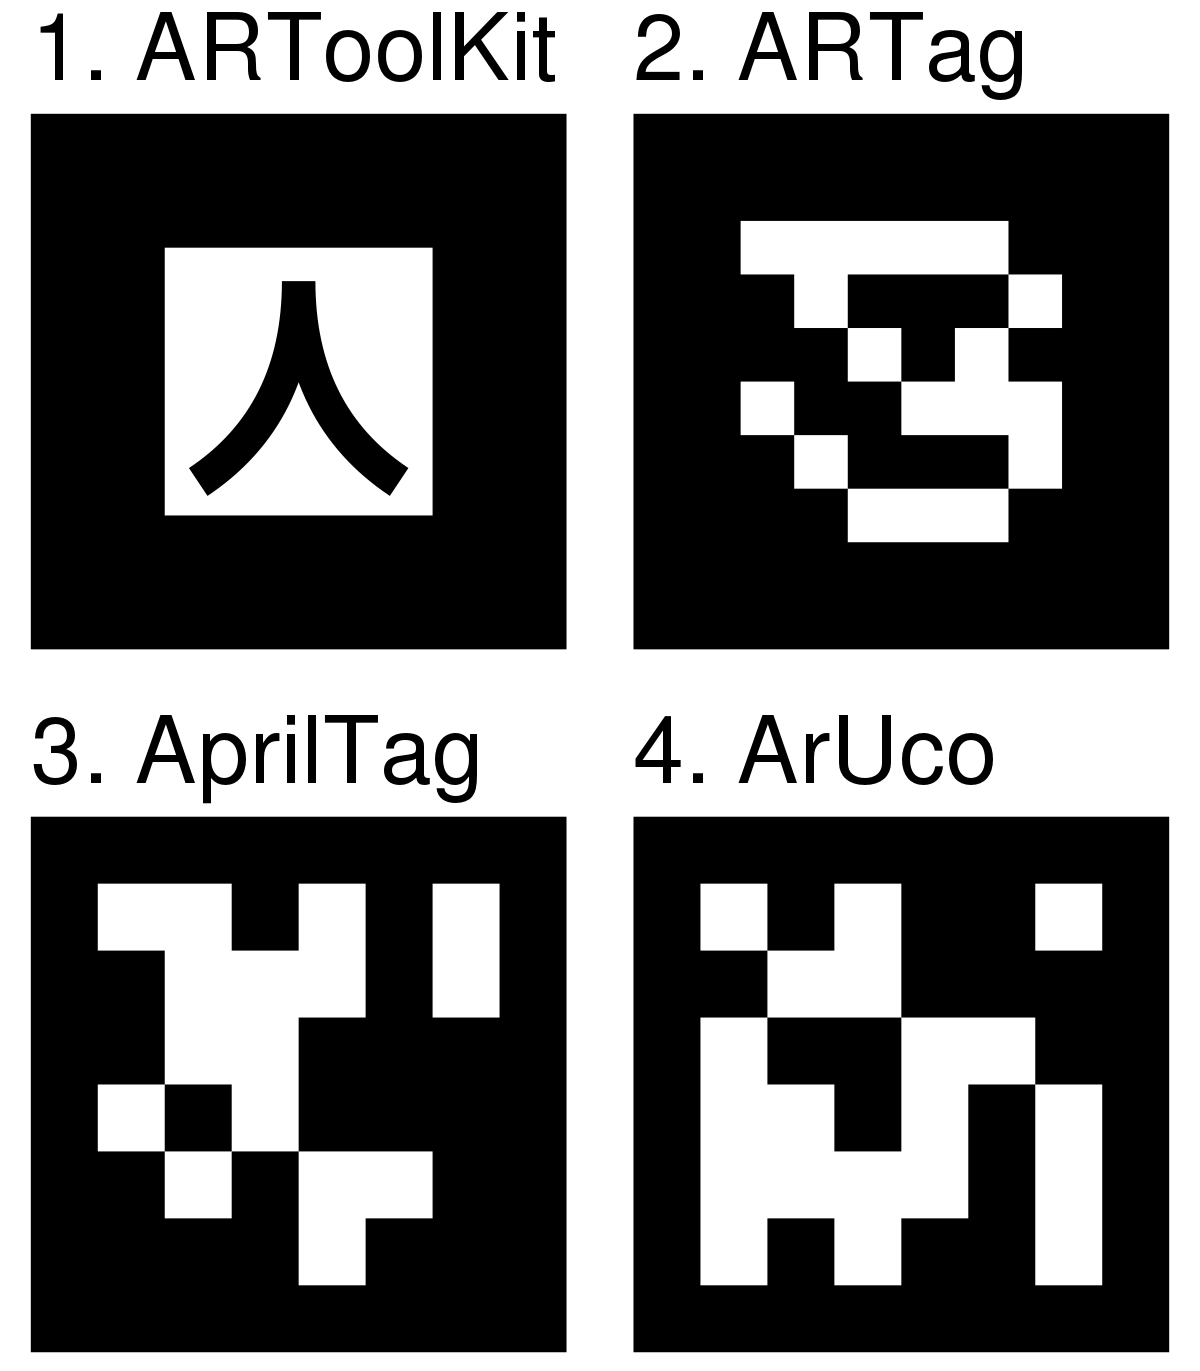
\includegraphics[width=3truecm, height=3truecm]{images/markerek.png}
	\caption{ArToolKit, ARTag, AprilTag, ArUco}
\end{figure}


\SubSection{Betanítható markerek}

A kiterjesztett valóság technikai fejlődéssel a markerek is bonyolultabbá váltak, lehetőség nyílt hétköznapi tárgyak, épületek és egyéb dolgok markerként kezelésére.

Természetesen ezek detektálása nehezebb, illetve betanítást igényel.

Léteznek továbbá úgynevezett marker nélküli (markerless) AR alkalmazások is, a szenzorok felmérik környezetet és megfelelő helyre pozicionálják a megjelenítendő objektumot/objektumokat. (pl. földrajzi koordináták felhasználása: PokemonGO)

\Section{Inerciális szenzorok}
Az inerciális szenzorok gyorsulásérzékelőkből, giroszkópokból magnetométerekből állnak.

\Section{Az Aruco marker használata}

Az ArUco (Augmented Reality University of Cordoba) markereket 2014-ben fejlesztette ki kollégáival S.Garrido-Jurado Spanyolországban. 

Az ArUco könyvtár nyílt forráskódú és C++ nyelven íródott, OpenCV alapú. 
Ar ArUco markerek két részből állnak, egy fekete keretből és egy egyedi bináris mintából, ami azonosítja a markert.

Az OpenCV-s támogatottsága miatt került kiválasztásra a dolgozathoz. A detektálást számos beépített függvény segíti.\\

\begin{figure}[htp]
    \centering
   	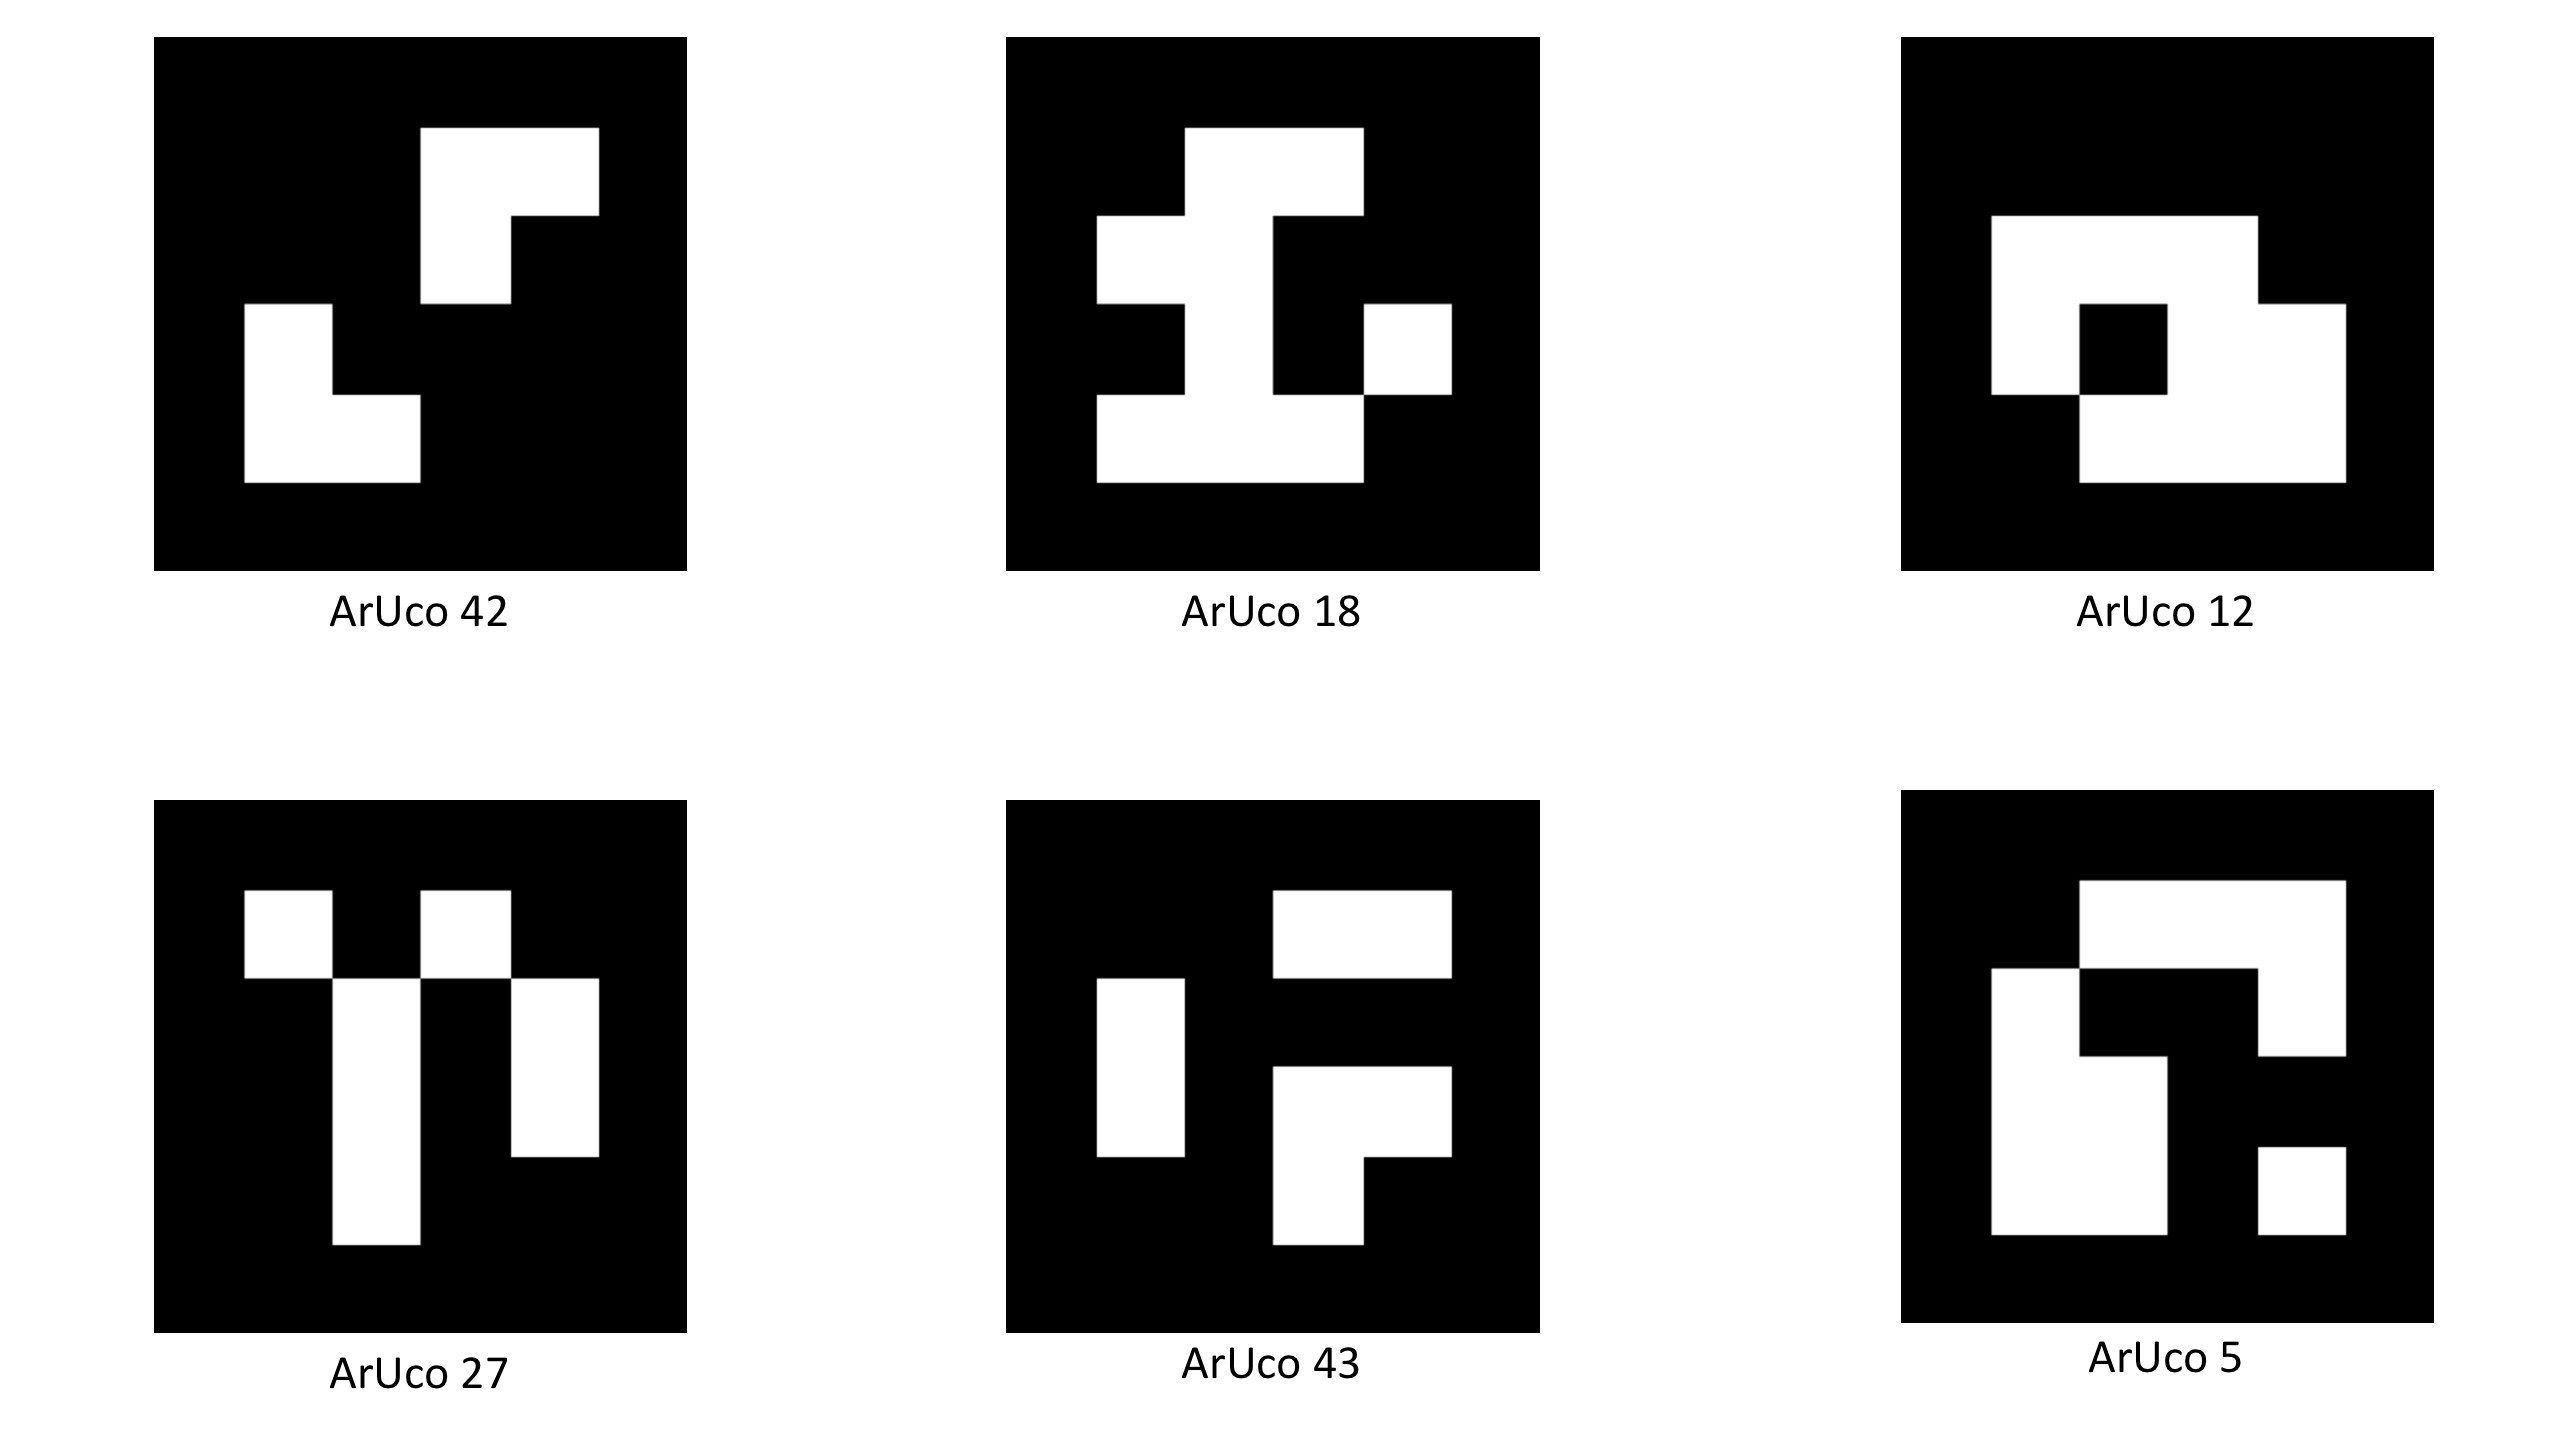
\includegraphics[width=4.8truecm, height=3truecm]{images/kep.png}
	\caption{Aruco markerek a 4X4-es könyvtárból}
\end{figure}

\SubSection{Típusai, használati módok}

Az ArUco markerek különböző könyvtárak érhetőek el, a minta mérete és belső mindta oszlop és sor száma tér el.

A bináris minta  4x4 mérettől a 7x7 méretig elérhető ( ez a belső mint a és ezekhez, 50, 100, 250, 1000 az oldalméret ez mm-ben értendő).

Azonban minél bonyolultabb egy minta és minél nagyobb annál nehezen felismerni, ezért én a  \texttt{DICT\_4X4\_100}-t használtam.

\SubSection{Kamera kalibrálása}

% TODO: https://medium.com/@aliyasineser/aruco-marker-tracking-with-opencv-8cb844c26628

A kamera kalibrációjához 6x9-es sakktábla mintát használtam. (A külső sáv nem számolandó bele, az a felismerést könnyíti, a belső minta számít.) 

A kalibráció eredményességéhez a négyzeteknek szabályosnak, egyformának kell lenniük és fontos, hogy a nyomtatás során a minta ne torzuljon el, ne legyen átméretezve. 

A pontosság növelése érdekében a képeket érdemes minél változatosabb szögben és távolságból elkészíteni. Valamint ügyelni kell arra, hogy a lap egyenes legyen, ezért célszerű megfelelő támaszt használni hozzá.

A kalibráció során kapjuk meg a későbbiekben nélkülözhetetlen együttható (kamera) mátrixot, a disztorziós együtthatókat, az eltolási és forgatási vektorokat.

A kalibrációt végző függvénynek a sorok és oszlopok számára, a négyzetek oldalhosszára és a fent említett képekre van szüksége.

A folyamat során meg kell határozni a sakktábla minta sarokpontjait \\
\texttt{findChessboardCorners()} függvénnyel, pontosabbá tenni azok koordinátáit \\
\texttt{cornerSubPix()} -lel. Majd ezen pontokat, (projekciós pontjai a sakktáblába mintának) a objektum pontjait ( a minta pontjai a minta terében), a kép méretét kell megadni \texttt{calibrateCamera()} függvénynek. \\

\begin{python}
  ret, mtx, dist, rvecs, tvecs = cv2.calibrateCamera(objpoints,
   imgpoints, gray.shape[::-1], None, None)
\end{python} 

A kimenetei a függvénynek:
\begin{itemize}
\item {\bf cameraMatrix}: $3 \times 3$ lebegőpontos kamera matrix
\[
A = 
\begin{bmatrix}
	f_x & 0 & 0 \\
	0 & f_y & 0 \\
	0 & 0 & f_z \\
\end{bmatrix}
\]

\item {\bf distortionCoefficient}: Bemeneti/kimenti torzítási együttható vektora:
\[
(k_1, k_2, p_1, p_2, [, k_3 [, k_4, k_5, k_6, [, s_1, s_2, s_3, s_4 [, \tau_x, \tau_y]]]])
\]
4, 5, 8, 12 vagy 14 elemből állhat.

\item {\bf rvecs}: A mintákhoz tartozó elforgatási vektorok becsült kimeneti vektora.

\item {\bf tvecs}  A mintákhoz tartozó vektorok becsült kimeneti vektor
\end{itemize}


\begin{figure}[htp]
    \centering
   	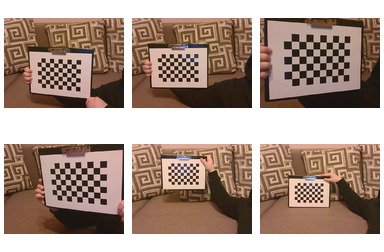
\includegraphics[width=7truecm, height=6truecm]{images/calibration.jpg}
	\caption{Kalibráláshoz használt képek közül néhány}
\end{figure}
%https://docs.opencv.org/master/d9/d0c/group__calib3d.html
%https://medium.com/@aliyasineser/opencv-camera-calibration-e9a48bdd1844

\SubSection{Demo alkalmazás}

A markerek detektálását befolyásolja a fényviszony, a kamerához viszonyított pozíció, a minta bonyolultsága, a szög amiben látszik és a mérete. Továbbá óriási hátrány, hogy ha takarásra kerül egy része a markernek, akkor nem lesz felismerhető.

Az ArUco marker felismerésére használt demó alkalmazás bekalibrálja a kamerát (ha ez még nem történt meg), majd a kalibrációból kapott \texttt{camera\_matrix} és a \texttt{dist\_Coefficient} felhasználásával detektálja a markert az élő képen.

A folyamatos kapcsolat érdekében végtelen ciklust indul. Majd kapcsolatot kell teremteni a kamerával és mindig az adott pillanatnyi képpel dolgozni. 
Meg kell adni a megfelelő könyvtárat, amiben szerepel a marker, amit fel akarunk ismerni. Jelen esetben ez  \texttt{DICT\_4X4\_100}.
\begin{python}
aruco_dict = aruco.Dictionary_get(aruco.\texttt{DICT\_4X4\_100})
\end{python}

Majd ezt a változót,a paramétereket, a képet, a kamera mátrixot és disztorziós együtthatókat felhasználva detektáljuk a markert a \texttt{aruco.detectMarker()} függvény segítségével.

\begin{python}
corners, ids, rejectedImgPoints = aruco.detectMarkers(image, aruco_dict,
parameters=parameters,
cameraMatrix=mtx,
distCoeff=dist)
\end{python}

Eredményként a sarok pontokat, forgásvektorok és eltolási vektorok tömbjét kapjuk meg, amik a markerre való rajzolásnál kapnak majd nagyobb szerepet.

Ha talál a képen markert a program, akkor körbe rajzolja azt, kijelöli a felső sarok pontját és ráteszi a képre marker koordináta rendszeréhez tartozó triédert.\\

\begin{python}
rvec, tvec ,_ = aruco.estimatePoseSingleMarkers(corners,
0.17, matrix_coefficients, distortion_coefficients)       
aruco.drawAxis(frame, matrix_coefficients, distortion_coefficients, 
rvec, tvec, 0.01)
\end{python}
\begin{figure}[htp]
    \centering
   	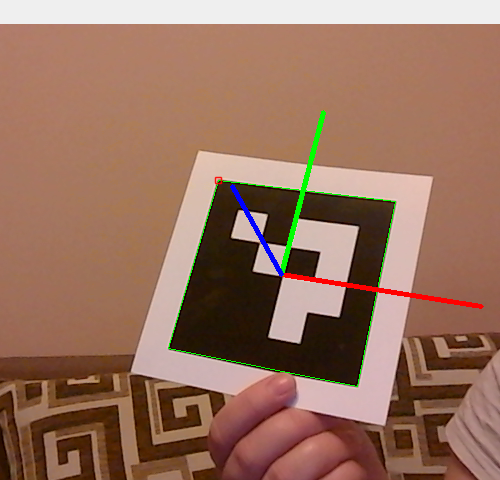
\includegraphics[width=4truecm, height=2.8truecm]{images/felismeres_aruco.png}
	\caption{A demó eredménye}
\end{figure}

\SubSection{A marker felismerésére készített program tesztje:}

A programban az ArUco marker felismerés egy olyan függvényként jelenik meg, ami megkap egy képet és ha talál rajta markert, akkor visszaadja a megfelelő vektorokat. (forgás és eltolás)

Ezen programrésznek a tesztelésére készítettem a nyomtatott markeremről pár képet és megnéztem milyen eredményeket ad vissza és felismeri-e a képen szereplő markert.

Azon kijelentés, hogy ha takarásba kerül a marker bármely része, akkor nem lesz továbbá felismerhető teljesen helytálló, hisz legyen bármilyen kicsi az eltakart rész a program nem ismeri fel. 

A képek, ahol felismerte a markert:

\begin{figure}[htp]
    \centering
   	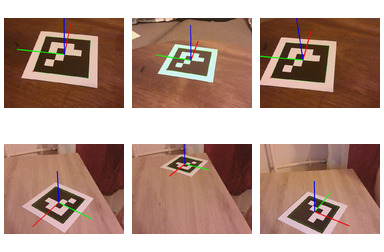
\includegraphics[width=6truecm, height=4.8truecm]{images/detect.jpg}
	\caption{sikeres detektálás}
\end{figure}


A képek, ahol nem ismerte fel a markert:
\begin{figure}[htp]
    \centering
   	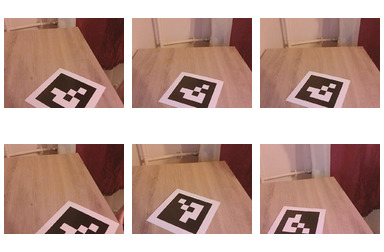
\includegraphics[width=6truecm, height=4.8truecm]{images/not_detect.jpg}
	\caption{sikertelen detektálás}
\end{figure}

